% Auditable-evaluation revision; source case rather than cell is the transfer unit.
\documentclass[preprint,12pt]{elsarticle}
\usepackage{amsmath,amssymb,booktabs,array,graphicx,placeins,float,url,hyperref}
\setlength{\emergencystretch}{2em}
\journal{Applied Energy}
\begin{document}
\begin{frontmatter}
\title{Auditable cross-source evaluation of battery lifetime predictions and restricted timing proxies}
\author[aff1]{[First Author]\corref{cor1}}
\ead{[corresponding.author@email]}
\cortext[cor1]{Corresponding author}
\affiliation[aff1]{organization={[Department, University]}, country={[Country]}}
\begin{abstract}
Archive endpoints, observation grids and censoring can change interpretations of battery lifetime scores. We evaluated 429 cells from six sources; cycle-100 source-held-out analysis included 376 cells and 228 endpoint events. Five survival methods used common source-only Brier tuning. An executable audit links event times, feature availability, scoring support and restricted timing losses. CALCE's lognormal accelerated failure-time model has integrated Brier score (IBS) 0.013 on a 125--500-cycle grid with one event. Its full-event median error is 5284\%. All 77 HUST archive labels differ from the end-of-life at 80\% capacity (EOL80) proxy, and TJU model ordering depends on the confirmation rule. Correcting frozen external scoring on 47 ISEA/RWTH cells changes event-time, integration and risk-direction interpretations. Separate canonical refits give cycle-100 XGBoost IBS 0.056, concordance 0.594 and event median error 30.8\%, versus KM IBS 0.114 and median error 6.9\%. Nested source-only selection compares median error, IBS and restricted timing loss across fixed windows and penalty ratios. At a 1000-cycle window with penalty ratio four, decision-based and IBS-based selection both choose forest externally; decision-based selection has higher loss than median-error-based selection by 0.207 (95\% conditional paired interval 0.176--0.234). These post hoc scenarios establish criterion-dependent decisions and adverse transfer outcomes rather than operating-cost savings. Processed-input availability, censoring assumptions and single-source external scope remain explicit.
\end{abstract}
\begin{keyword}
battery cycle life \sep data provenance \sep cross-source transfer \sep right censoring \sep endpoint sensitivity \sep survival evaluation
\end{keyword}
\end{frontmatter}

\section{Introduction}

Battery lifetime studies require evaluation that preserves the meaning of the predicted endpoint across measurement and cycling protocols. Early-life prediction, state of health (SOH) transfer and heterogeneous-data curation motivate traceable source-level comparisons \citep{severson2019,attia2020,attia2026,wang2024pin,tang2024ae,ledeng2026,zhu2026lake}.

Cross-dataset prediction failure is already documented. Schauser et al. evaluate Severson-style feature-based linear models across Voltaiq Community datasets and identify poor extrapolation, feature overfitting and unphysical lifetime predictions \citep{schauser2022}. Survival and probabilistic battery prognosis are also established. Santhira Sekeran et al. model censored lifetime with AFT and transfer between chemistries using target labels \citep{sekeran2022}. Ly et al. evaluate KM-weighted non-crossing quantile LSTM prediction on simulated hourly trajectories with synthetic training censoring \citep{ly2023}. Ibraheem et al. use early voltage-path signatures and gradient-boosted Cox models on measured cells, reporting concordance, dynamic AUC and IPCW Brier scores under batch-stratified splits \citep{ibraheem2025}. Vasilev et al. analyze survival-metric sensitivity to event distributions, time bins and censoring imbalance in medical data \citep{vasilev2023}. BatteryLake supplies provenance and curation for SOH and remaining useful life (RUL); its preprint distinguishes registered from fully curated datasets \citep{zhu2026lake}. Supplementary S6 distinguishes these tasks, inputs and evaluation designs. Their scores are not matched benchmarks for the capacity summaries used here.

Three challenges motivate the present evaluation. First, archive lifetime labels, capacity thresholds and observation rules can define different endpoints. Second, a supported probability-scoring window can contain too few events to assess full-lifetime predictions; favorable window scores need not establish accurate event-time medians. Third, model selection by prediction error or probability score need not select the same actions as an explicit restricted timing loss, and transfer conclusions can depend on the action window. We test these dependencies through a joint endpoint--information--support--decision contract.

\begin{samepage}
The study makes three contributions.
\begin{enumerate}
\item An executable audit connects source provenance, observed-record endpoints, feature timing and scoring support across six archives and one separate processed-series archive (Sections 2.1--2.4; Supplementary S1, S7 and S11).
\item A common-objective, source-held-out comparison of five survival methods isolates metric and endpoint dependence, with target-cell and training-sample uncertainty assessed separately (Sections 3.1--3.4 and 3.6; Supplementary S2, S3 and S8).
\item A nested source-only comparison of median-error, IBS and decision-loss selection links predictions to a restricted timing proxy and retains adverse, zero and unavailable outcomes across the full scenario grid (Section 3.5; Supplementary S11--S14).
\end{enumerate}
\end{samepage}
The contribution concerns evaluation choices and their evidenced consequences. The six internal archives are source-level transfer cases. ISEA/RWTH adds one separate source for prediction evaluation; its decision scenarios were designed after examining that source and remain exploratory.

\section{Materials and methods}
\subsection{Source provenance and observed-record endpoint}
The corpus contains 124 MIT, 55 XJTU, 130 TJU, 34 unique NASA, 9 CALCE and 77 HUST cells. Source articles and repositories are cited separately \citep{severson2019,wang2024pin,wang2024dataset,zhu2022tju,zhu2022dataset,saha2007,calce2026,calcek2,he2011calce,ma2022hust,ma2022hustdata}. Selected local source files, hashes, unit conversions and exclusions are recorded in the audit package. NASA cathode chemistry cannot be certified from the available local metadata. CALCE combines reported lithium cobalt oxide (LCO) and lithium iron phosphate (LFP) subsets. TJU mAh readings were converted to Ah and incomplete discharge records excluded. HUST source RUL and the present end-of-life at 80\% capacity (EOL80) proxy disagree for all 77 cells; they are distinct targets. Source identity confounds chemistry, temperature, test protocol and follow-up length.

For cell $j$, $Q_j(c)$ is valid capacity at cycle $c$ and $\mathrm{SOH}_j(c)=Q_j(c)/Q_j(c_{j,0})$, where $c_{j,0}$ is the first valid observation rather than a nominal rated capacity. The primary target is the first of three consecutive \emph{observed} records with SOH $\leq0.8$. The integer cycle numbers need not be adjacent. A cell without a qualifying run is right-censored at its last valid observation. This is an observed-record EOL80 \emph{proxy}, not a certified physical failure time. Event time is assigned retrospectively to the first low reading; an online alarm is available only at the third confirming reading. One- and five-observation rules and a strict three-reading rule requiring adjacent integer cycles are sensitivity endpoints. The per-cell observation audit reports gaps, confirmation cycles and delays.

At landmark $L\in\{50,100\}$, a cell must be observed event-free past $L$, and features use records at or before $L$. The cycle-100 cohort contains 376 cells, 228 events and 148 censored observations; the cycle-50 cohort contains 379 cells, 230 events and 149 censored observations. Of 34 NASA cells, 11 had an endpoint by cycle 100 and 15 had no later follow-up, leaving eight eligible cells. Figure~\ref{fig:cohort} summarizes the overall research framework and the cycle-100 cohort; Supplementary S1 gives eligibility by source. A median record-density value near 1.000 describes coverage of the \emph{processed cycle-record grid}. Instrument sampling cadence is a separate source characteristic (Supplementary S1).

\begin{figure}[htbp]\centering
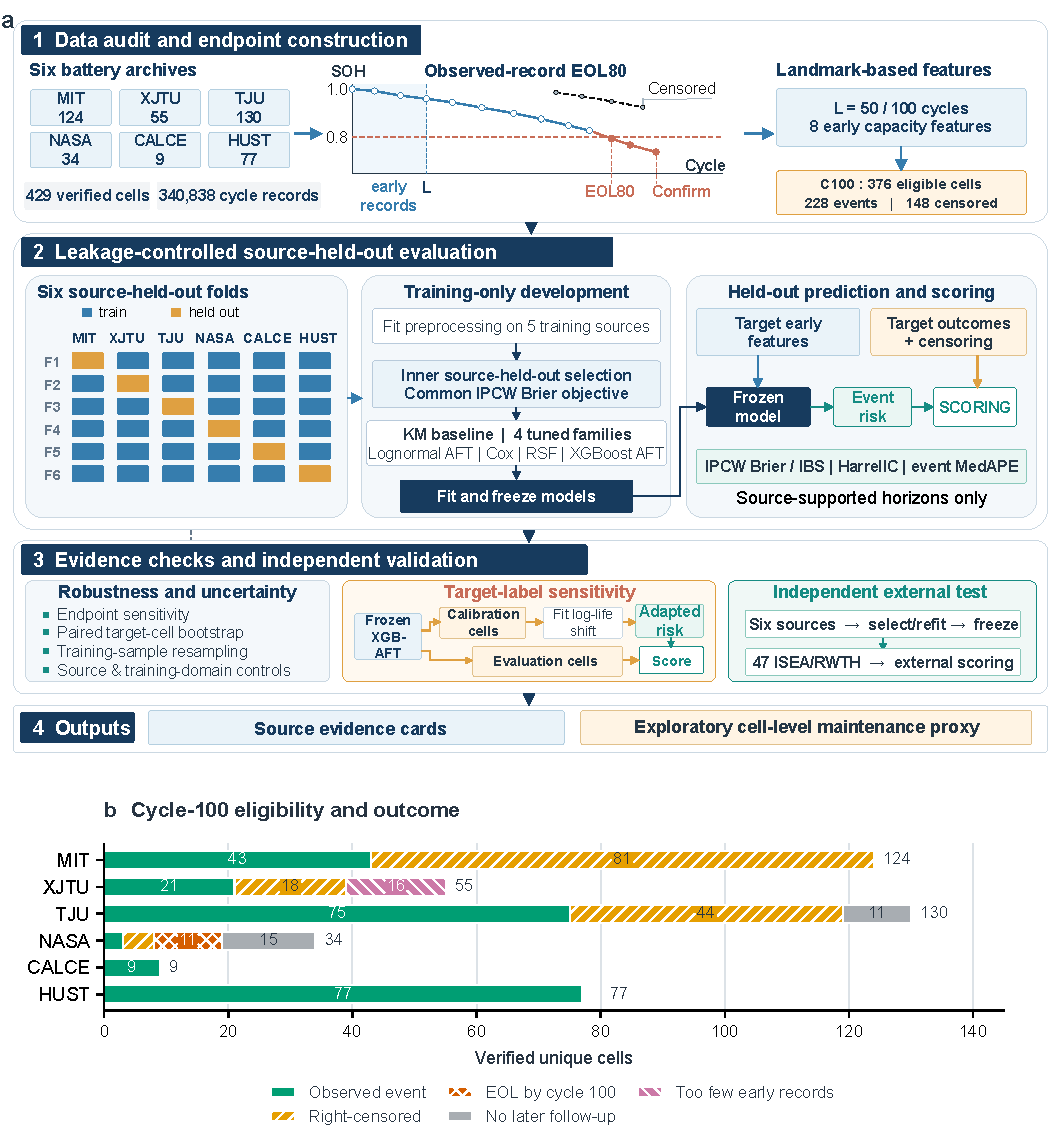
\includegraphics[width=0.90\linewidth,height=0.72\textheight,keepaspectratio]{../figures_v6/fig_v6_source_cohort.pdf}
\caption{Overall auditable research framework and the six-source cycle-100 cohort. (a) SOH curves are schematic: features use records at/before $L$; EOL80 is the first of three consecutive observed lows, confirmed at the third. Matrix columns follow the listed source order: five train and one held out. Preprocessing and inner IPCW Brier selection use training sources only. Separate branches show endpoint, uncertainty and target-label sensitivities; target calibration and evaluation cells are distinct. External models are selected/refit on all six sources and frozen before ISEA/RWTH scoring. KM is untuned; four families are tuned. Outputs are source evidence cards and a restricted endpoint-timing proxy with source-only median, IBS and decision selection. External evaluation concerns processed series; timing-proxy scenarios are post hoc. Schematic trajectories are not measured observations. (b) Cycle-100 eligibility/outcomes. End labels give archive totals; segment counts appear for at least nine cells. Internal sources are transfer cases.}\label{fig:cohort}
\end{figure}

\subsection{Landmark survival models and common model selection}
For eligible cells, remaining life is $R=T-L$ and residual follow-up is $Y=\min(T,C)-L>0$. An observed event contributes $f_R(Y\mid x)$ to a continuous likelihood and censoring contributes $S_R(Y\mid x)$. For lognormal accelerated failure time (AFT), $\log R=\mu(x)+\sigma Z$, $Z\sim N(0,1)$, so the event risk at absolute cycle $t>L$ is
\begin{equation}F(t\mid x,T>L)=\Phi\left(\frac{\log(t-L)-\mu(x)}{\sigma}\right).\end{equation}
Eight early capacity features include first valid capacity, landmark SOH, early slope, two drops, variability and two recovery measures. Training-fold imputation and scaling prevent preprocessing leakage. The models are pooled-source Kaplan--Meier (KM) without cell features \citep{kaplan1958}, regularized lognormal AFT, regularized Cox \citep{cox1972}, random survival forest (RSF) \citep{ishwaran2008}, and XGBoost AFT. For Cox, survival is evaluated as $\widehat S(t\mid x)=\exp[-\widehat H_0(t)\exp\{\eta(x)\}]$ in the log domain; invalid or unconverged fits remain unavailable and are never probability-clipped. The release path is versioned \texttt{v6.2-b0-nearest-feasible-20261010} with an input and code fingerprint recorded in the reproduction receipt. Pooled-source KM is fitted on the five training sources in each outer fold; it does not use labels from the held-out source.


For records $(c_i,s_i)$ available by $L$, let $\bar c$ and $\bar s$ denote record means and $d_i=s_{i+1}-s_i$. Features are: first valid capacity $q_0$ (Ah); last available SOH; $1000\sum_i(c_i-\bar c)(s_i-\bar s)/\sum_i(c_i-\bar c)^2$ (SOH per 1000 cycles); $1-s$ at the last record at/before cycle 10 and $\lfloor L/2\rfloor$; population SOH standard deviation; count of $d_i>0.001$; and signed $\max_i d_i$. Missing early drops use training-only imputation. Record rises do not identify a physical regeneration mechanism. Supplementary S11 gives exact fields and units.

Each outer fold holds out one source. Candidate parameters for all four tuned model families are selected using the \emph{same} mean IPCW Brier objective over the common supported horizons of each inner source-held-out fold. The inner selection uses only the five training sources; no outer-target outcome selects a candidate. The horizon grid is absolute cycle 125, 250, 500, 750, 1000, 1500 and 2000. The held-out source supplies its censoring KM only for evaluation \citep{gerds2006}; horizons with inadequate censoring or observation support are unavailable. Within a source the five methods share one supported horizon grid. Source-specific trapezoidal integrated Brier scores (IBS) are compared within a row, not pooled across different source grids. Harrell's concordance \citep{harrell1982} describes ranking. Event-cycle median absolute percentage error (MedAPE) is $100\operatorname{median}_{i\in\mathcal E_f}\left(\frac{|\widehat T_i-T_i|}{T_i}\right)$, where $\widehat T_i=L+\operatorname{median}(\widehat R_i)$ and $\mathcal E_f$ contains observed events with finite predicted medians. The denominator is absolute event cycle $T$, rather than remaining life $T-L$. Supplementary S12 reports finite-median counts against all observed events; partial availability affects the population summarized by this error. The source-level marginal censoring KM requires independent censoring within that source; conditional independence given features alone does not establish validity of these marginal weights. This assumption is not verifiable from the archives.

\subsection{Uncertainty, endpoint and target-label controls}
For each source, we resample target cells 2000 times with the same cell indices for every model, recompute censoring weights, and score the \emph{original fixed horizon grid}. Draws lacking full support are recorded as unavailable; all scored draws use the original grid. We compute paired IBS differences for all ten model pairs at both landmarks; the displayed XGBoost AFT-minus-KM and forest-minus-KM contrasts retain the same cells and weights. We report exploratory, unadjusted 95\% pointwise percentile intervals conditional on fixed predictions and the held-out source. NASA has no integrated score. We also report risk set size and censor survival at each supported horizon.

A separate cycle-100 sensitivity resamples cells within each of the five training sources, preserving source sample sizes, and refits XGBoost AFT and pooled KM 200 times per estimable target. Source-selected configuration, seed 0, target cells and target scoring horizons remain fixed; no target labels select or adapt a predictor. The 2.5th--97.5th percentile ranges describe training-sample sensitivity conditional on full support in both models. These sensitivity analyses were added post hoc. Protocol records document the analysis settings and input hashes.

One-, three-, five-observation and strict adjacent-cycle EOL80 rules are refitted with Cox and XGBoost AFT on a common cohort using the source-selected parameters from the primary three-observation analysis. The scored horizon grid is intersected across all four rules in each source. The analysis compares model ordering across four explicitly defined outcomes. Source-correction contrasts evaluate the joint training-table changes on identical verified evaluation cells and labels. At cycle 100, 2000 paired target-cell bootstrap draws use the same sampled cells for both frozen training branches and model families, recompute censoring weights and retain the full original horizon grid. Pointwise percentile intervals describe source-conditional target-cell variability; draws lacking full grid support are unavailable. Within-archive batch dependence and retraining variation are outside this resampling model.

Within-source out-of-fold XGBoost AFT and XJTU/TJU group-held-out XGBoost AFT are descriptive training-domain controls. Target-source labels are available to the within-source arm, and group training sizes differ from the source-held-out arm. TJU group and chemistry differences coincide, so a protocol-specific effect cannot be isolated. Event-only regression is a label-availability control: it fits source events but borrows the source-selected AFT scale to construct a probability \emph{proxy}. Its Brier result is conditional on that borrowed scale.

For exploratory target adaptation, target cells with frozen source-held-out XGBoost AFT predictions are randomly assigned without event stratification to $m=\lceil pn\rceil$ calibration cells and the remaining evaluation cells, where $p=0.10,0.20,0.40$. A one-parameter log-remaining-life shift is fitted by censored likelihood; its prior scale is selected within the five source-validation domains only. Sensitivity is evaluated across 30 overlapping calibration/evaluation draws and 20 training seeds on the same target cells. Split-specific evaluation-cell bootstrap intervals additionally condition on the fitted model, selected calibration cells and fitted shift. Supplementary S4 evaluates the event-label counts required by the specified event-only 95\% empirical-quantile construction \citep{angelopoulos2021}.

\subsection{External prediction evaluation and exploratory decision analysis}
The ISEA/RWTH P001 input \citep{isea2021}, stored in a MATLAB structure named \texttt{TDS}, comprises 47 numbered cells on a provider-processed five-cycle capacity grid. All 10,686 sample rows were checked: 3,510,013 overlapping cycle values agree exactly. A verified crosswalk to the separately supplied 48 named P001 cells is unavailable. The local preprocessing code starts from this supplied structure and does not establish upstream smoothing/interpolation or online availability. External conclusions therefore concern the supplied processed series. Features remain at/before the landmark; this restriction alone does not certify upstream online availability.

The outcome contract stores last observation, event, confirmation, analysis-stop and last-feature cycles separately. An event is scored at EOL80, not terminal follow-up; censoring is scored at the last observation. Larger risk means earlier endpoint. IBS is the normalized trapezoidal Brier integral; the equal-horizon Brier mean is retained solely as the tuning objective. Frozen historical predictions are rescored separately from new fits. The latter use one Python 3.11 dependency lock and six source-validation folds at each landmark, each trained on the other five sources, followed by a full six-source refit. Historical risk recovery uses an explicitly separate Python 3.12 environment and reproduces stored probabilities.

For replacement evaluation, $H\in\{500,1000,1500\}$, $U=\min(T,H)$, planned cycle $A$, and effective cycle $a=\min(A,H)$ define
\begin{equation}\ell_H(a,T)=\frac{(U-a)_++\rho(a-U)_+}{H-L}.\label{eq:replacement}\end{equation}
This dimensionless endpoint-timing penalty is a scenario proxy. We use $\rho\in\{1,2,4,8\}$ and maintenance opportunities every 25, 50 or 100 cycles from $L$, including $H$. Reference settings are $L=100$, $\rho=4$, and 50-cycle opportunities; $L=50$ is a sensitivity. Planned actions beyond $H$ mean continued operation within the window. At $H$, continued operation and replacement have equal restricted timing loss, so action flags are reported separately. A constant replacement cost common to all policies cannot establish a gain.

Distribution policies minimize
\begin{equation}\widehat E[\ell_H(a,T)\mid x]=\frac{\int_a^H\widehat S(t\mid x)\,dt+\rho\int_L^a[1-\widehat S(t\mid x)]\,dt}{H-L}\end{equation}
on common opportunities, with exact step/lognormal integrals and earlier-action numerical ties. B0 selects the feasible opportunity nearest to cycle 1000 for each $(L,H,\delta)$, with earlier ties; B1 chooses a fixed cycle using source validation; B2 is pooled-KM distribution minimization, identical to KM-Pd. Pm maps the predicted median to the nearest opportunity, using a recorded B1 fallback if unavailable; Pd minimizes the distribution loss. Oracle $a=U$ is only a zero-loss evaluation bound.

S-M, S-I and S-D choose the family by source-validation MedAPE, IBS and Pd loss. Each outer target is excluded from all fitting and selection. Each inner validation source is also excluded from its hyperparameter selection, which uses the remaining sources. The primary S-I, S-M and S-D comparison uses one common intersection of estimable validation sources, with equal source weights and fixed family-order ties. A separately labelled loss-only S-D sensitivity uses the broader timing-loss support; it is not a pure metric contrast with the matched primary criteria. This is a selection heuristic, not a pooled-population IBS ranking. For censored targets, known $U$ contributions use marginal reverse-KM weights $1/G(Y-)$ for observed events by $H$ and $1/G(H)$ for follow-up covering $H$; $H$-early censoring is not assigned an endpoint. Weight survival below 0.10 or insufficient prediction/validation support yields NA. Complete external events use direct loss means. Decision estimability at $H=1500$ is separate from conservative IBS-grid support.

All 504 source/landmark/scenario combinations are retained. Paired 2000-cell draws fix models and selected families and reestimate censoring weights; S-D-minus-S-I and S-D-minus-S-M are designated analysis contrasts, with pointwise conditional intervals. These scenarios were designed after examining ISEA and are exploratory. Source-only fitting and family selection protect the prediction/selection layer, but do not provide independent confirmation of target-informed scenario design. Conditional cell-bootstrap intervals do not account for that design choice. The previous derating replay is retained as historical context in Supplementary S9; it cannot identify an independent derating benefit.
\section{Results}
\subsection{Six source-held-out benchmark cases}
Table~\ref{tab:main} shows cycle-100 IBS after common-objective tuning. Different methods attain the lowest point score in different source cases: forest on MIT and TJU, XGBoost AFT on XJTU and HUST, and lognormal AFT on nine CALCE cells. CALCE's lognormal AFT has IBS 0.013 over cycles 125, 250 and 500, with cumulative event counts 0, 0 and 1 among nine cells. Its full-event MedAPE is 5284\%. These measures assess different targets: probabilities inside the supported window and medians of the complete event-time distribution. A zero-risk diagnostic gives IBS 0.037 on the same grid, so the fitted model improves this window score; the improvement does not establish useful lifetime medians. Supplementary S2 gives the point scores and diagnostic calculation. NASA has eight eligible cells and three events. Its only supported horizon is cycle 125, so its Brier scores provide single-horizon descriptions. NASA provides neither an IBS comparison nor an estimable target decision-loss comparison under the specified support rules. Supplementary S2 reports conditional intervals and horizon support for these point rankings.

The separate fully nested endpoint-refit audit also exposes finite far-tail predictions on CALCE. At L100, the native one-observation cohort has seven events and lognormal AFT MedAPE 31905.8\%, MAE 111075.3 cycles and MedAE 40520.4 cycles; its predicted residual-life median across events is 40547.4 cycles. On the seven-event common cohort under the three-observation rule, MedAPE remains 3508.4\%, MAE 37742.9 cycles and MedAE 20313.8 cycles; predicted residual-life median is 20792.8 cycles. These are distinct refits and cohorts from Table~\ref{tab:main}. The latter events have residual lifetimes 309--553 cycles, so their large error cannot be attributed solely to events near the landmark or a remaining-life denominator. Across 14 correlated target/landmark blocks on matched support, choosing MAE, MedAE or median symmetric absolute percentage error instead of MedAPE changes the error-selected family in 6, 4 and 4 blocks; the corresponding disagreements with S-I are 10, 10 and 9. No metric is established as universally preferable.

The HUST archive's source RUL label encodes its own terminal cycle, whereas our endpoint is the first of three observed SOH readings at or below 0.8. The two cycle labels differ for \emph{all 77 HUST cells}; the source terminal cycle is later by a median of 258 cycles (range 104--524). HUST results therefore concern the reconstructed EOL80 proxy, not prediction of the archive's original RUL target.

\begin{table}[htbp]\centering\small
\caption{Cycle-100 source-held-out integrated IPCW Brier score. N/E is eligible cells/observed events; "Cycles" is the supported scoring-horizon range, not the observed cell-life range. Best-score 95\% intervals resample cells with frozen predictions and are conditional on the single held-out source. Lower scores are better within a row only. NA: one supported horizon, so no integral. KM: pooled-source Kaplan--Meier; LN-AFT: lognormal AFT; RSF: random survival forest.}\label{tab:main}
\begin{tabular*}{\linewidth}{@{\extracolsep{\fill}}lcccccc}\toprule
Source & N/E & KM & LN-AFT & Cox & RSF & XGB-AFT \\\midrule
MIT &124/43&0.163&0.175&0.185&\textbf{0.139}&0.155\\
XJTU &39/21&0.058&0.203&0.078&0.065&\textbf{0.055}\\
TJU &119/75&0.325&0.207&0.180&\textbf{0.155}&0.190\\
NASA &8/3&NA&NA&NA&NA&NA\\
CALCE &9/9&0.040&\textbf{0.013}&0.102&0.177&0.285\\
HUST &77/77&0.259&0.179&0.168&0.307&\textbf{0.153}\\\bottomrule
\end{tabular*}
\vspace{2mm}

\begin{tabular*}{\linewidth}{@{\extracolsep{\fill}}lccc}\toprule
Source & Supported scoring cycles & Horizons & Best-score 95\% CI \\\midrule
MIT &125--1000&5&0.108--0.170\\
XJTU &125--500&3&0.022--0.091\\
TJU &125--1000&5&0.136--0.179\\
NASA &125 only&1&NA\\
CALCE &125--500&3&0.000--0.034\\
HUST &125--2000&7&0.132--0.176\\\bottomrule
\end{tabular*}
\end{table}

The paired contrasts in Table~\ref{tab:paired} qualify the point rankings. Both displayed MIT contrasts and the XJTU XGBoost AFT-minus-KM contrast have intervals crossing zero. Forest has a positive difference on XJTU; both contrasts are positive on CALCE. The negative TJU differences and HUST XGBoost AFT difference concern these particular source cases and scoring grids.
Figure~\ref{fig:benchmark} visualizes the source-held-out point scores and conditional intervals on their source-specific supported grids.
\begin{table}[htbp]\centering\small
\caption{Cycle-100 paired IBS differences relative to pooled-source KM. Entries give point difference [95\% pointwise cell-bootstrap interval]; negative favors the named model. The same target draws, frozen predictions and full original grid are used for both models. These post hoc contrasts are not adjusted for multiple comparisons. Valid counts and all ten pairs at both landmarks are in Supplementary S2.}\label{tab:paired}
\begin{tabular*}{\linewidth}{@{\extracolsep{\fill}}lcc}\toprule
Source & XGB-AFT minus KM & RSF minus KM \\\midrule
MIT & -0.008 [-0.016, +0.001] & -0.024 [-0.050, +0.002]\\
XJTU & -0.002 [-0.009, +0.004] & +0.007 [+0.003, +0.011]\\
TJU & -0.134 [-0.171, -0.092] & -0.170 [-0.191, -0.139]\\
NASA & NA & NA\\
CALCE & +0.245 [+0.164, +0.333] & +0.137 [+0.055, +0.220]\\
HUST & -0.106 [-0.139, -0.071] & +0.048 [+0.041, +0.057]\\
\bottomrule\end{tabular*}\end{table}

\begin{figure}[htbp]\centering
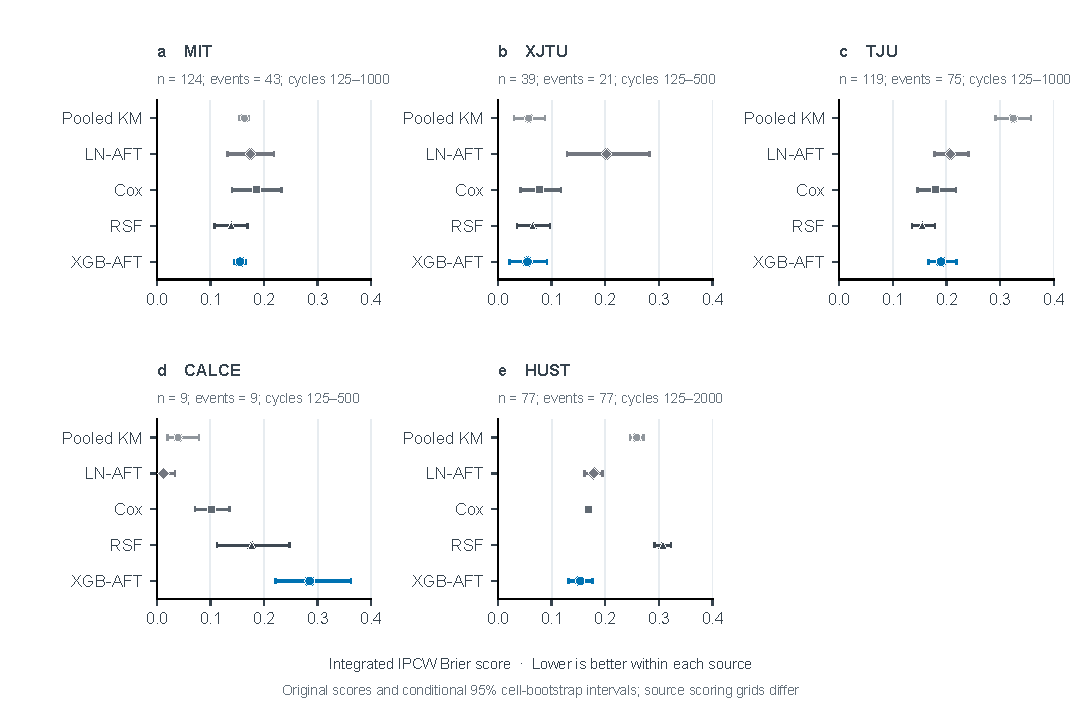
\includegraphics[width=\linewidth]{../figures_v4/fig_v4_benchmark_brier.pdf}
\caption{Five-model source-held-out benchmark after common-objective inner tuning. Points show original IBS; whiskers show 95\% percentile cell-bootstrap intervals conditional on fixed predictions and the held-out source. Comparisons use a common scoring grid within each source; grids differ between sources. NASA is omitted from this IBS panel because only cycle 125 is supported and no IBS is estimable. Pooled KM: pooled training-source Kaplan--Meier; LN-AFT: lognormal AFT; RSF: survival forest; XGB-AFT: XGBoost AFT.}\label{fig:benchmark}
\end{figure}

Horizon-level risk can disagree even when integrated error is modest. For XGBoost AFT at cycle 500, CALCE's mean predicted event risk is 0.690, compared with a held-out KM risk of 0.111. At cycle 2000, HUST values are 0.208 and 0.896. Only eight HUST cells remain at risk beyond that horizon. Figure~\ref{fig:risk} shows every supported horizon, and Supplementary S2 records each risk set and censor weight.
\begin{figure}[htbp]\centering
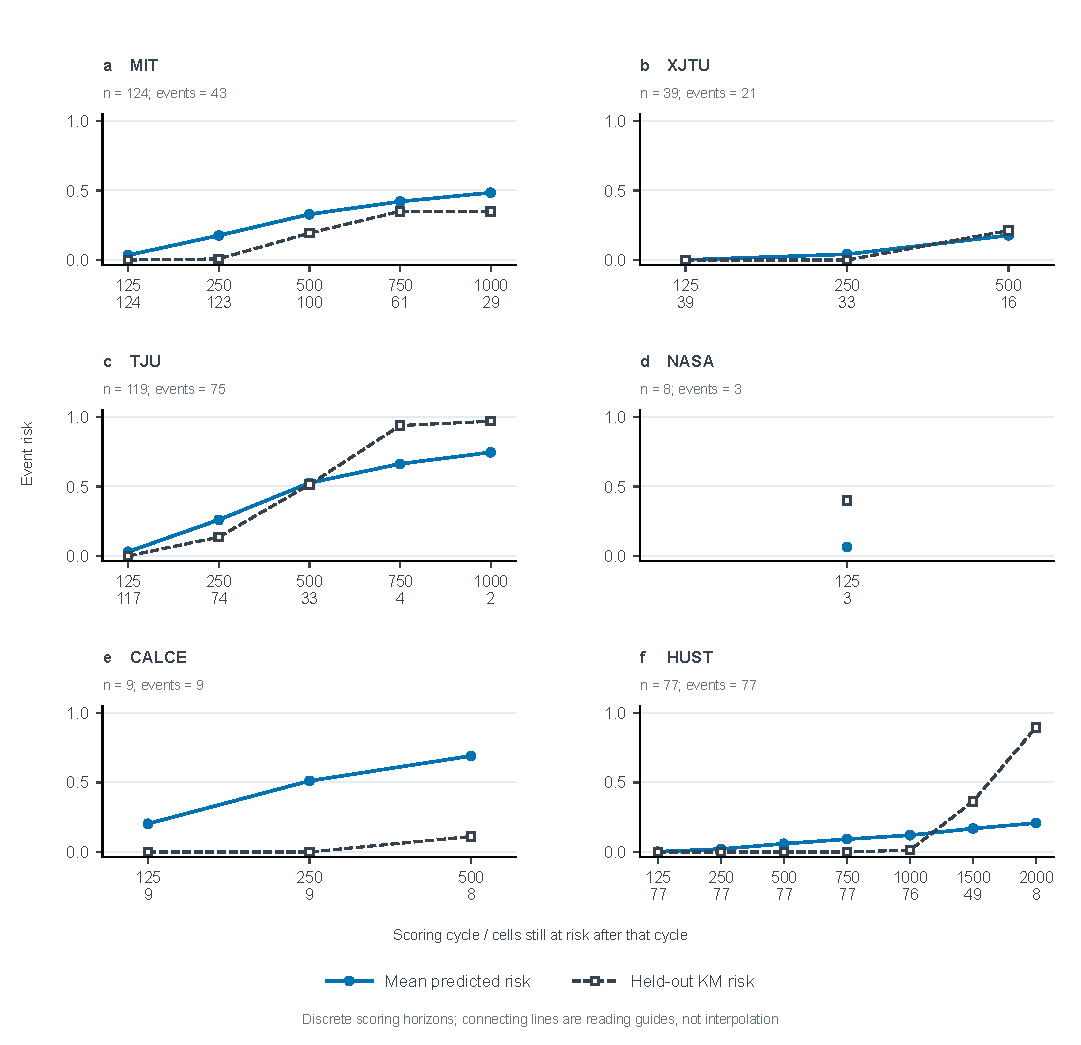
\includegraphics[width=\linewidth]{../figures_v4/fig_v4_survival_calibration.pdf}
\caption{Mean XGBoost AFT event risk and held-out KM event risk at each supported cycle-100 scoring horizon. All panels share the risk scale. Tick labels give the scoring cycle above and the number of cells still at risk after that cycle below. Horizons are discrete categories with equal visual spacing; connecting lines guide reading and do not interpolate risk between horizons. These fold-level diagnostics are not individual calibration curves.}\label{fig:risk}
\end{figure}

\subsection{Endpoint and provenance sensitivity}
The one-, three-, five-observation and strict adjacent-cycle comparison uses 374 cycle-100 cells across all six sources eligible under the one-observation restriction. XJTU retains the same 39 test cells, 21 three-observation events and cycle-125/250/500 scoring grid as Table~\ref{tab:main}. Its IBS of 0.059 here versus 0.055 in Table~\ref{tab:main} comes from separate refits under different training cohorts: the common-cohort restriction removes two CALCE training cells. The endpoint observation audit found three cells whose strict and observed three-reading endpoints differ: one each in XJTU, TJU and NASA. In a controlled MIT observation-grid replay at landmark 100, retaining every processed record yielded 43/124 confirmed events, a 5-cycle grid yielded 34/124, and a 20-cycle grid yielded 0/124; the corresponding right-censoring fractions were 0.653, 0.726 and 1.000. The 5-cycle grid delayed the 34 commonly confirmed events by a median of 9 cycles, while the 20-cycle grid had no estimable confirmation delay. These are changes in the observed-record endpoint and support contract, not claims that physical failures disappeared. With fixed predictions, support-matched S-I selected RSF/Cox/Cox and S-M selected Cox/Cox/Cox at 1/5/20-cycle grids. Forcing all three grids to use common validation sources and scoring horizons left S-I and S-M at Cox/Cox/Cox; that common set contains only unchanged CALCE, TJU and XJTU, excluding intervened MIT. Probability-only S-I also remained Cox/Cox/Cox. The loss-only S-D sensitivity selected RSF/RSF/Cox. Complete nested refits for the ISEA outer target selected S-I/S-M/S-D as RSF/RSF/XGB-AFT at 5 cycles and RSF/Cox/Cox at 20 cycles; S-D here uses loss-only support. Refitting changes both training labels and fitted distributions and is not a pure fixed-prediction measurement effect. Confirmation requires at least two further cycle records and can take longer when records are skipped. Strict refitting changes XJTU XGBoost AFT IBS on the common grid from 0.05937 to 0.05954. By contrast, XJTU's one-, three- and five-observation targets have 24, 21 and 16 events and XGBoost AFT scores 0.091, 0.059 and 0.049 on the paired cohort. These are different outcome definitions. Figure~\ref{fig:endpoint} summarizes the resulting score and ordering sensitivity; full per-source event, lag and score tables are in Supplementary S3.
\begin{figure}[htbp]\centering
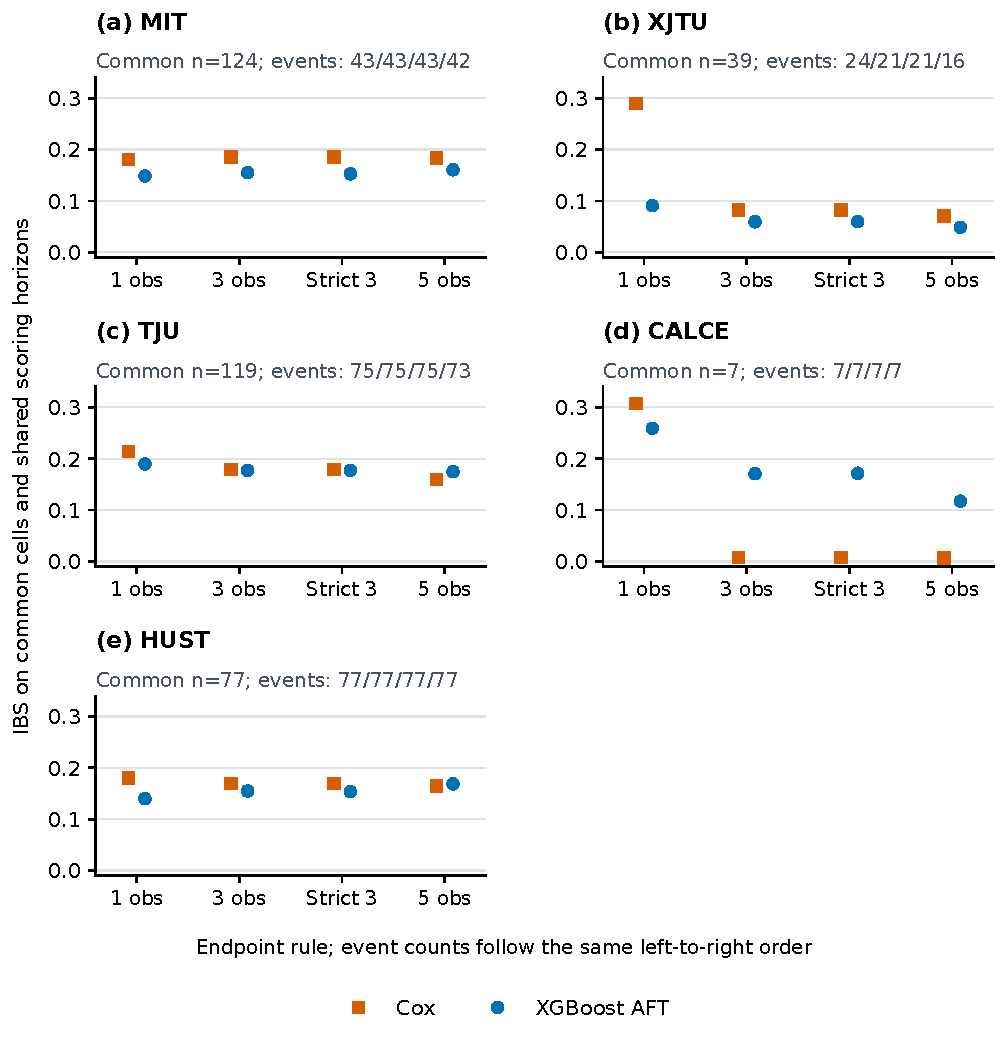
\includegraphics[width=\linewidth]{../figures_v4/fig_v4_endpoint_model_sensitivity.pdf}
\caption{Endpoint sensitivity on common cells and shared scoring horizons: one, three and five consecutive observed low-SOH records, and the strict adjacent-integer-cycle three-record rule (Strict 3). The five plotted sources share the IBS scale; NASA is omitted because no IBS is estimable under its single supported horizon. Event counts follow the endpoint order shown on the axis. Each rule defines a separate outcome; the panels compare sensitivity of model scores and ordering to that definition. Strict-rule refits and the full numerical results are reported in Supplementary S3.}\label{fig:endpoint}
\end{figure}

Corrected training records change errors in both directions on fixed verified test labels. For XGBoost AFT, CALCE IBS changes from 0.203 to 0.285, while HUST changes from 0.156 to 0.153. The contrast evaluates the joint training-table corrections on fixed test cells and labels. Figure~\ref{fig:correction} shows the paired training-table contrast. The CALCE XGBoost AFT difference is +0.0819 (95\% pointwise interval [+0.0467, +0.1115]); the HUST difference is -0.0027 [-0.0056, +0.0003]. The HUST interval spans zero despite its lower point estimate. Supplementary S10 reports all contrasts.
\begin{figure}[htbp]\centering
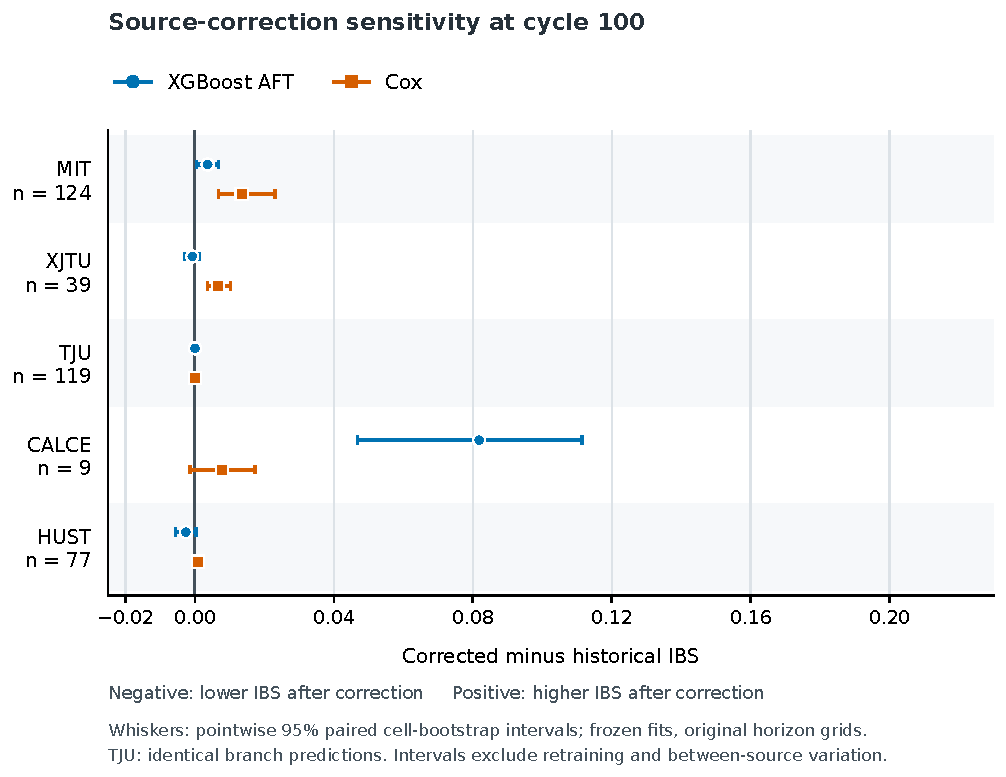
\includegraphics[width=\linewidth]{../figures_v4/fig_v4_source_correction.pdf}
\caption{Corrected-minus-historical-training IBS at cycle 100 on the same verified target cells and labels. Points show original differences; whiskers show pointwise 95\% paired cell-bootstrap intervals conditional on frozen fits and the full original scoring grid. Negative values favor corrected training. TJU has identical branch predictions; NASA is omitted because one supported horizon cannot provide an IBS contrast. All 2000 draws are valid except TJU (1780). These exploratory contrasts evaluate joint training-table corrections; numerical intervals and the resampling protocol are in Supplementary S10.}\label{fig:correction}
\end{figure}

\subsection{Training-domain and target-label controls}
At cycle 100, within-source XGBoost AFT IBS is lower than source-held-out XGBoost AFT on MIT (0.070 versus 0.155), TJU (0.165 versus 0.190), CALCE (0.118 versus 0.285) and HUST (0.150 versus 0.153), but higher on XJTU (0.087 versus 0.055). These arms differ in label access and training size. XJTU group-held-out IBS is 0.058 versus source-held-out IBS of 0.055; the corresponding TJU scores are 0.247 versus 0.190. The group contrast jointly reflects chemistry, protocol and training-size differences. Supplementary S4 reports event-only regression as a label-access sensitivity control using the borrowed AFT scale.

At the 20\% target budget, calibration counts are MIT 25, XJTU 8, TJU 24, NASA 2, CALCE 2 and HUST 16. In 30 seed-0 draws, a shifted model has lower paired IBS in 29, 6, 13, unavailable, 30 and 30 draws, respectively. Across 20 seeds crossed with the same draws, mean paired differences (shifted minus unshifted) are $-0.0186$ MIT, $+0.0076$ XJTU, $+0.0040$ TJU, unavailable NASA, $-0.0486$ CALCE and $-0.0125$ HUST (Supplementary S4). These means summarize conditional sensitivity across overlapping draws. Each CALCE shift uses two calibration cells. Split-specific bootstrap intervals condition on the fitted model, calibration membership and fitted shift. Figure~\ref{fig:recal} displays the paired IBS sensitivity across the overlapping target-cell splits.
\begin{figure}[htbp]\centering
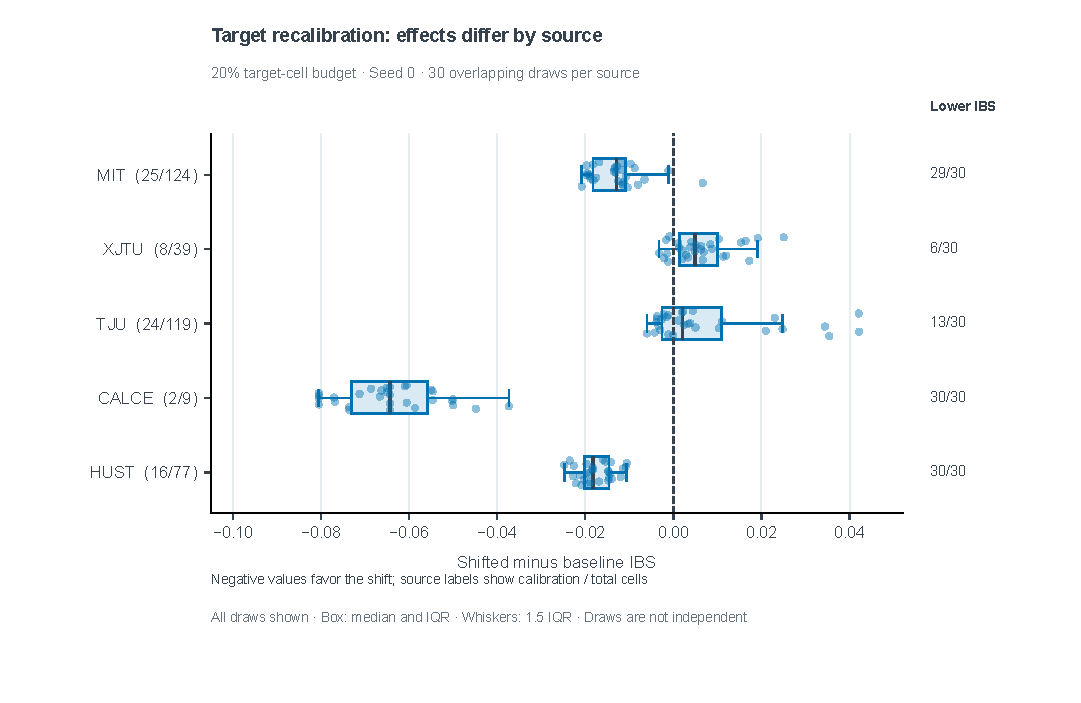
\includegraphics[width=\linewidth]{../figures_v4/fig_v4_target_recalibration.pdf}
\caption{Seed-0 paired 20\% target-cell shift sensitivity over 30 overlapping draws, on one common horizontal scale. Dots show all draws; boxes show the median and interquartile range, with whiskers extending to the furthest draw within 1.5 interquartile ranges. Counts at right give draws with lower IBS. Source labels give calibration/total cells. Negative values favor the shift. The box plots summarize sensitivity across overlapping splits of the same target cells under fixed source models. NASA is omitted because one supported horizon cannot provide an IBS contrast.}\label{fig:recal}
\end{figure}

The 20\% target-label budget often lacks enough observed event residuals even to compute the specified finite empirical quantile. The calculation evaluates event-label count feasibility for the specified 95\% empirical quantile; Supplementary S4 reports the exact probabilities.

\subsection{Independent external validation}
Table~\ref{tab:external} distinguishes corrected frozen scores from canonical v6.2 refits. All 47 processed-series endpoints are observed, but only cycles 125, 250, 500, 750 and 1000 satisfy the conservative scoring-support rule. Three endpoints occur by 1000, none by 500, and all lie between 920 and 1360. Terminal observations are 445--590 cycles later than EOL80. Historical terminal-time scoring, equal-horizon averaging and inverted risk ordering were corrected jointly. This is a scoring repair, not a gain from retraining.

The canonical cycle-100 XGB-AFT IBS is 0.056 with C=0.594 and MedAPE 30.8\%, whereas KM MedAPE is 6.9\%. The feature-based models have C=0.594--0.617, indicating limited individual discrimination on this source. Their concordance point estimates alone do not establish equivalence to random ranking. KM gives tied predictions and C=0.500 by construction. A probability-score advantage does not establish a median-life advantage. Figure~\ref{fig:external_decision} shows paired contrasts for both versions; source-specific uncertainty does not estimate variation across new external archives.


\begin{table}[H]\centering\scriptsize
\caption{Cycle-100 external scoring on the same 47 cells and five supported horizons. Frozen: historical predictions after scoring correction; v6.2: independent canonical refits with landmark-specific six-fold source tuning. Median error concerns observed events.}\label{tab:external}
\begin{tabular*}{\linewidth}{@{\extracolsep{\fill}}llllll}\toprule
Model & Frozen IBS & Frozen C & v6.2 IBS & v6.2 C & v6.2 MedAPE (\%)\\\midrule
KM & 0.114 & 0.500 & 0.114 & 0.500 & 6.9\\
LN-AFT & 0.075 & 0.610 & 0.070 & 0.617 & 12.0\\
Cox & 0.070 & 0.611 & 0.070 & 0.611 & 14.1\\
RSF & 0.208 & 0.618 & 0.160 & 0.602 & 46.6\\
XGB-AFT & 0.054 & 0.592 & 0.056 & 0.594 & 30.8\\
\bottomrule\end{tabular*}\end{table}


\begin{figure}[htbp]\centering
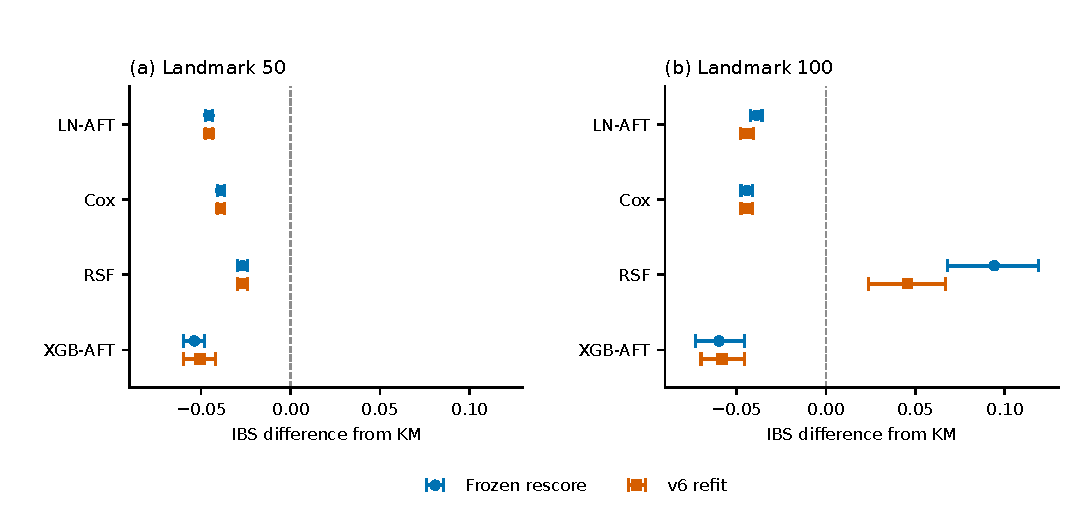
\includegraphics[width=\linewidth]{../figures_v6/fig_v6_external_scoring.pdf}
\caption{External model-minus-KM IBS differences for frozen rescoring and canonical refits. Both landmark panels use the same 47 cells and cycles 125/250/500/750/1000. Bars are 95\% pointwise paired percentile intervals from 2000 target-cell draws with fits fixed; negative favors the model. These intervals condition on this single processed-series source.}\label{fig:external_decision}
\end{figure}
\subsection{Source-only selection and replacement timing}
At the reference settings, selection criteria disagree on several source cases (Figure~\ref{fig:selection}). ISEA's S-M chooses Cox, while S-I and S-D choose RSF. Their common validation set contains MIT, XJTU, TJU and CALCE; B1 additionally uses HUST. In the HUST outer fold the common set contains only MIT and CALCE. Supplementary S13 reports source identities, exclusions and winner--runner-up gaps. ISEA's reference gaps are 0.38045 percentage points for S-M (Cox versus RSF), 0.00241995 IBS for S-I (RSF versus Cox), and 0.02885089 loss for S-D (RSF versus KM). These are point-selection margins, not probabilities of stable selection. The paired loss intervals fix selected families and do not include reselection variation. S-D-minus-S-I loss is zero because their actions coincide. S-D-minus-S-M is +0.207 [0.176, 0.234], retaining an adverse external result despite source-side decision selection. Only 3/47 endpoints occur within the 1000-cycle window. For the other 44 complete events, $U=H$ and B0 has $a=H$, yielding zero restricted loss. This is truncation of the loss window, not right censoring of their observed lifetimes. Earlier action incurs $(H-a)/(H-L)$ for those cells, so this window structurally favors continued operation on most of the cohort. B0 loss is 0.017 with 3/47 late actions; B1 and B2 loss is 0.551 with no late actions. RSF selection loss is 0.696 and Cox selection loss is 0.489, both with no late actions. Avoiding the three late actions thus incurs a substantial early-timing penalty under this scenario. The S-D versus S-M difference is entirely earlier action: both have zero late timing, while S-D adds 186.2 mean early cycles, giving 186.2/900 = 0.207 additional loss.

At $H=500$, no endpoint is observed within the window; any apparent advantage there concerns unnecessary early action and cannot validate near-endpoint risk detection. At $H=1500$, all 47 endpoints are within the window and the three reference selection rules coincide. Figure~\ref{fig:tradeoff} separates these windows. NASA target loss remains unavailable under inadequate censoring support; unavailable outcomes are not filled with terminal times or zero losses. Supplementary S14 maps all external penalty/opportunity combinations and summarizes all seven targets, retaining positive, zero, negative and unavailable contrasts. At L100/H1000, D-minus-M is positive in six settings and zero in six; at L50/H1000 it is negative in one and zero in eleven. At L100/H1000, D-minus-I is negative in seven and zero in five, whereas at H1500 it is positive in five and zero in seven. These overlapping scenarios are descriptive sensitivity cases, rather than independent tests or evidence of a universally best criterion.

\begin{figure}[htbp]\centering
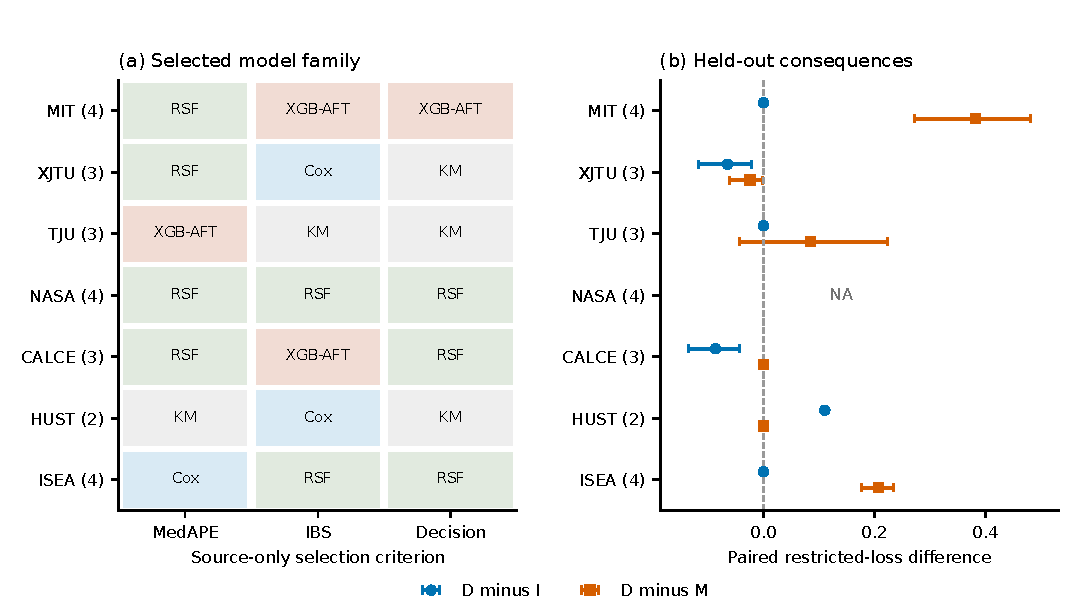
\includegraphics[width=\linewidth]{../figures_v6/fig_v6_selection_consequences.pdf}
\caption{Family selection and its held-out consequences at L=100, H=1000, rho=4 and 50-cycle opportunities. (a) Source-only selected families; each source label gives its common validation-source count. Identities and exclusions are in Supplementary S13. (b) S-D-minus-S-I and S-D-minus-S-M restricted-loss differences, with 95\% pointwise paired conditional intervals from 2000 cell draws; NASA target loss is NA. Negative favors decision-based selection. All three criteria use the same estimable source intersection within each outer fold.}\label{fig:selection}
\end{figure}

\begin{figure}[htbp]\centering
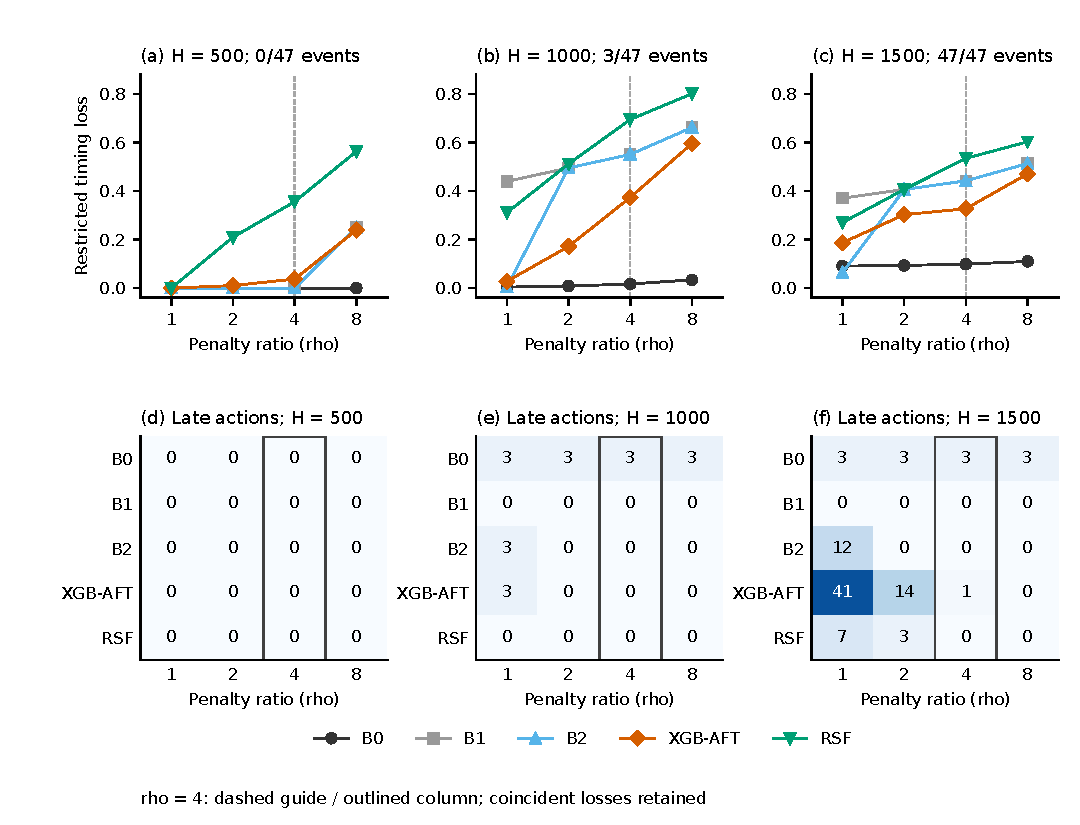
\includegraphics[width=\linewidth]{../figures_v6/fig_v6_replacement_tradeoff.pdf}
\caption{Penalty-ratio sensitivity on 47 complete external events at L=100 and 50-cycle opportunities. Panels (a--c) show loss at four equally spaced discrete $\rho$ categories (1, 2, 4, 8); colors and markers identify policies. Connecting segments are visual guides between evaluated scenarios. Panels (d--f) give exact late-action counts; shading uses the same 0--47 range. A dashed guide and outlined column mark $\rho=4$. Coincident losses remain overlapping without jitter; Supplementary Table S19 lists every value. Windows are separate restricted estimands; this displayed reference slice does not select an optimal scenario. Points are original scenario means; paired conditional intervals and the full 25/50/100-cycle grid are supplied in the aggregate tables. B2 is identical to KM-Pd. No endpoint occurs by H=500.}\label{fig:tradeoff}
\end{figure}
On the common 119-cell TJU endpoint cohort, source-selected primary configurations are frozen while outcomes are refitted under one, three, five and strict-three records. The shared scoring grid is intersected across all rules and models. In this conditional sensitivity, S-D changes from RSF under one record to RSF under three and KM under five; confirmation timing remains separate from the retrospectively assigned event. The primary full-cohort analysis and the common-cohort sensitivity are distinct fits. A separate HUST sensitivity changes only its training target to the archive RUL terminal target, retaining common features, configurations and held-out EOL80 scoring. HUST-held-out predictions are identical because neither branch trains on HUST labels. This establishes a computational target-definition contrast, not an error in the provider's target or a physical-failure claim.
\subsection{Audit findings that change interpretation}
Table~\ref{tab:judgment} links measurements to the conclusions they support. At TJU, XGBoost AFT has lower IBS than Cox for the one- and three-observation outcomes (0.190 versus 0.214 and 0.177 versus 0.179), but Cox has lower IBS for the five-observation outcome (0.159 versus 0.175). All use common cells and the intersected grid; the change identifies endpoint dependence rather than performance improvement on an unchanged target.
\begin{table}[htbp]\centering\small
\caption{Audited evidence and its consequences for interpretation of the six-source benchmark.}\label{tab:judgment}
\begin{tabular}{@{}>{\raggedright\arraybackslash}p{26mm}>{\raggedright\arraybackslash}p{48mm}>{\raggedright\arraybackslash}p{50mm}@{}}\toprule
Audit & Observed evidence & Consequence for interpretation \\\midrule
Metric meaning & CALCE LN-AFT IBS 0.013 on a three-point grid with one event; full-event MedAPE 5284\% & Window probability accuracy does not establish useful full-event lifetime medians.\\[3pt]
Label semantics & HUST: 77/77 labels differ; archive terminal cycle later by median 258 cycles & Results concern reconstructed EOL80, not the archive RUL target.\\[3pt]
Endpoint rule & TJU Cox/XGB ordering reverses for five observations; XJTU events change 24/21/16 & State the outcome rule with each comparison; score reductions across rules are not gains on one outcome.\\[3pt]
Support and adaptation & NASA has one horizon; CALCE shift uses two labels; XJTU/TJU mean shift differences are positive & Report NASA at its single supported horizon and evaluate adaptation separately for each source and calibration budget.\\\bottomrule
\end{tabular}
\end{table}

Training resampling adds variability excluded from the frozen-prediction intervals. At MIT, the fixed-configuration XGBoost AFT IBS ranges from 0.138 to 0.248 across the 2.5th--97.5th percentiles of 200 training draws. The paired XGBoost AFT-minus-KM ranges cross zero on MIT and XJTU. For HUST, 175/200 draws preserve full support in both models; 25 lack the pooled-KM training follow-up needed for the original cycle-2000 horizon and are unavailable. The ranges are conditional on this support restriction. Supplementary S8 reports all sources.

Executable consistency checks confirm that the within-source and group-control frozen references reproduce the current benchmark labels and predictions; the within-source protocol's recorded input hashes match current files. The endpoint script reads the current selected configurations. Supplementary S5 and S8 specify the verified code/input links, recorded hashes and historical record availability.

\subsection{Release-path and stability audit}
The stable Cox implementation was promoted into the shared Bank path before this release evaluation. In a clean Python 3.11 environment, ten fresh external fits reproduced the cached risk scores and survival curves within $10^{-7}$; the benchmark configurations and family winners were unchanged. Across the affected benchmark rows, the only score differences were floating-point changes of approximately $10^{-17}$ in Cox IBS. The isolated replacement replay produced no changes in selected families, planned actions, or timing-loss fields. These checks compare old and new outputs explicitly; they do not turn an invalid fit into a scored result.

Selection, predictive error and action stability are reported as separate objects. The release audit retains NA whenever event support, censoring support or a complete median is unavailable. In the strict common-support analysis, the historical source-level margin can still be formed by cancellation among sources; a small aggregate margin is not a selection probability. The observed endpoint is an observed-record EOL80 proxy. It does not confirm physical failure, intervention benefit, safety benefit or an economic return. The six archives also do not constitute a first cross-domain battery-lifetime benchmark with a common observation mechanism.\label{sec:release_audit}

\section{Discussion}
The audit answers the three research questions by separating metric interpretation, outcome dependence and available validation evidence. It complements curation and predictive-model research with a reproducible chain linking source records to supported conclusions. The CALCE diagnostic shows why sparse-window probability accuracy cannot certify full-event lifetime medians. HUST target labels change meaning, and the TJU comparison depends on the observation rule. These dependencies are documented in the six selected archives.


The external results constrain the practical value established for early capacity summaries. Feature-based concordance of 0.594--0.617 indicates modest discrimination among these 47 processed-series cells; XGB-AFT's lower IBS accompanies worse event-median error than pooled KM. Together with the adverse reference decision contrast, these results do not establish a stable ranking or operational advantage from adding the eight capacity features. The capacity summaries may omit informative voltage-path or operating-condition features. Source identity also confounds chemistry, temperature, cycling protocol and follow-up. The five-cycle provider grid and unverified upstream processing could alter early information, but their effect has not been isolated. These are candidate explanations requiring matched input and processing controls. The result concerns this one processed-series source and does not characterize all new battery sources.

The decision comparison additionally depends on the endpoint mass inside each window. At H=1000, 44/47 events lie beyond H and continued operation has zero restricted loss for those cells; at H=500 no endpoint enters the window. At H=1500 all events enter and the three reference selection rules coincide. The complete scenario inventory exposes this dependence but cannot remove the influence of having examined ISEA before defining the scenarios. The comparison therefore describes conditional consequences of source-only selection under exploratory losses. Confirmatory decision validation requires fixing the endpoint, windows, penalty ratios and opportunities before inspecting a new external source, followed by evaluation on that source. Operating-cost benefit additionally requires measured action costs and intervention outcomes.

The uncertainty assessment separates target-cell sampling, training-sample variation and variation across new sources. Target-cell bootstrap intervals hold trained models fixed; training-resampling ranges hold configurations and target cells fixed. These conditional assessments quantify different components and cannot be combined as one confidence interval. The ISEA/RWTH test adds one independent cell archive, with all 47 processed-series cells reaching the observed endpoint and five supported scoring horizons; population variation across additional sources remains unestimated. XJTU has four eligible batch labels and TJU has three eligible subsets within the same archives, with chemistry/protocol confounding in TJU. Calendar-time validation requires certified experiment start dates, which are unavailable in the current schema; cycle order describes follow-up within a cell. Failure-related test stopping could also violate independent censoring. The event-label feasibility calculation addresses the residual count required by a finite quantile; all-cell conformal coverage requires a separate censor-aware evaluation.

\subsection{Evidence needed before storage decisions}
For an energy researcher using a lifetime predictor in a subsequent study, the outputs specify concrete checks. An intervention study must name the capacity measurement, threshold and confirmation delay before interpreting predicted remaining life; HUST shows why archive RUL cannot be substituted automatically. A risk-constrained storage model must request probabilities only at supported horizons and examine risk-set sizes and horizon-level discrepancies; NASA cannot provide a multi-horizon score, and only two TJU cells remain at risk beyond cycle 1000. A transfer study must declare whether target labels are available and preserve a separate evaluation set; the CALCE shift is evaluated with two calibration cells per draw. The timing-proxy analysis tests whether source-only median, probability-score and decision-loss selection produce the same actions. The adverse ISEA reference contrast shows that optimizing this proxy on training sources does not establish a transferred maintenance benefit. A pack or dispatch simulation additionally needs a validated cell-to-pack mapping, operating load and held-out reliability/cost data. The source cards and decision protocol organize the evidence needed to design these subsequent studies.

Supplementary S7 gives a reusable source evidence card: provenance and endpoint, cohort/events, supported cycles and final risk set, horizon discrepancies, target-label budget, grouping and chronology, and the corresponding interpretation. It records the supported scoring horizons and marks unsupported requests as unavailable. The card organizes the evidence available for using a lifetime predictor in a subsequent system study. Its endpoint is capacity-based; physical failure and safety assessment require additional failure-related measurements \citep{attia2026}.

\section{Conclusion}
The six-source audit and independent ISEA/RWTH test identify four dependencies in battery lifetime evaluation: CALCE's sparse-window Brier minimum does not certify full-event median-life accuracy; HUST's reconstructed EOL80 differs from its archive RUL target for all 77 cells; the TJU Cox/XGBoost ordering changes with the observation rule; and the external source has a different relationship between IBS and event MedAPE under the frozen six-source fit. Common-objective selection, paired contrasts on fixed scoring grids, external testing and training resampling support source-specific comparisons with explicit conditional variability. Nested source-only timing-proxy selection exposes criterion-dependent actions and adverse transfer under an explicit restricted timing loss. These post hoc processed-series proxies do not establish operating-cost savings; pack mapping and operating-data validation remain required for system decisions.

\section*{Data availability statement}
Source archives remain with their original providers. Public v6.2 code, aggregate data and figures are released at \href{https://github.com/whuaying/auditable-battery-lifetime-evaluation}{github.com/whuaying/auditable-battery-lifetime-evaluation}; a permanent DOI deposit is pending. Cell/cycle-derived tables, model caches and provider archives remain local pending source-specific redistribution review. External replay requires the provider archives and documented parsers.
\section*{Declaration of competing interest}
To be completed and approved by all authors before submission.
\section*{CRediT authorship contribution statement}
To be completed from the actual author roles before submission.
\section*{Funding}
To be completed from verified funding records before submission.
\section*{Acknowledgments}
The authors acknowledge the public dataset providers.
\section*{Declaration of generative AI and AI-assisted technologies in the manuscript preparation process}
ChatGPT/Codex assisted with prose editing, code generation, computational checks and figure preparation. This declaration is a draft; all authors must review the output, confirm the tool-use description and approve the final responsibility statement before submission.
\begin{thebibliography}{99}

\bibitem[Severson et~al.(2019)]{severson2019}
Severson, K.~A., Attia, P.~M., Jin, N., Perkins, N., Jiang, B., Yang, Z., et~al. (2019). Data-driven prediction of battery cycle life before capacity degradation. \textit{Nature Energy}, \textit{4}(5), 383--391. \url{https://doi.org/10.1038/s41560-019-0356-8}

\bibitem[Attia et~al.(2020)]{attia2020}
Attia, P.~M., Grover, A., Jin, N., Severson, K.~A., Markov, T.~M., Liao, Y.-H., et~al. (2020). Closed-loop optimization of fast-charging protocols for batteries with machine learning. \textit{Nature}, \textit{578}(7795), 397--402. \url{https://doi.org/10.1038/s41586-020-1994-5}

\bibitem[Attia et~al.(2026)]{attia2026}
Attia, P.~M., Weng, A., \& Chueh, W.~C. (2026). Limits of electrochemical data for predicting battery lifetime and failure. \textit{Joule}, \textit{10}, 102423. \url{https://doi.org/10.1016/j.joule.2026.102423}

\bibitem[Wang et~al.(2024)]{wang2024pin}
Wang, F., Zhai, Z., Zhao, Z., Di, Y., \& Chen, X. (2024). Physics-informed neural network for lithium-ion battery degradation stable modeling and prognosis. \textit{Nature Communications}, \textit{15}, 4332. \url{https://doi.org/10.1038/s41467-024-48779-z}

\bibitem[Tang et~al.(2024)]{tang2024ae}
Tang, A., Xu, Y., Hu, Y., Tian, J., Nie, Y., Yan, F., Tan, Y., \& Yu, Q. (2024). Battery state of health estimation under dynamic operations with physics-driven deep learning. \textit{Applied Energy}, \textit{370}, 123632. \url{https://doi.org/10.1016/j.apenergy.2024.123632}

\bibitem[Le et~al.(2026)]{ledeng2026}
Le, H., Deng, W., Nguyen, K.~T.~P., Medjaher, K., Gogu, C., \& Wu, D. (2026). Physics-informed transfer learning by embedding physics into activation functions: An application in battery health management. \textit{Applied Energy}, \textit{406}, 127161. \url{https://doi.org/10.1016/j.apenergy.2025.127161}

\bibitem[Zhu et~al.(2026)]{zhu2026lake}
Zhu, T., Wang, H., \& Wen, Y. (2026). BatteryLake: Agentic, physics-grounded curation of heterogeneous battery aging data and benchmarking. \textit{arXiv preprint arXiv:2607.09762}. \url{https://doi.org/10.48550/arXiv.2607.09762}

\bibitem[Wang(2024)]{wang2024dataset}
Wang, F. (2024). Project -- physics-informed neural network for lithium-ion battery degradation stable modeling and prognosis [Dataset]. Zenodo. \url{https://doi.org/10.5281/zenodo.10963339}

\bibitem[Zhu et~al.(2022)]{zhu2022tju}
Zhu, J., Wang, Y., Huang, Y., et~al. (2022). Data-driven capacity estimation of commercial lithium-ion batteries from voltage relaxation. \textit{Nature Communications}, \textit{13}, 2261. \url{https://doi.org/10.1038/s41467-022-29837-w}

\bibitem[Zhu et~al.(2022)]{zhu2022dataset}
Zhu, J., Wang, Y., Huang, Y., et~al. (2022). Data-driven capacity estimation of commercial lithium-ion batteries from voltage relaxation [Dataset]. Zenodo. \url{https://doi.org/10.5281/zenodo.6405084}

\bibitem[Saha and Goebel(2007)]{saha2007}
Saha, B., \& Goebel, K. (2007). Battery data set. \textit{NASA Ames Prognostics Data Repository}. NASA Ames Research Center, Moffett Field, CA. \url{https://www.nasa.gov/intelligent-systems-division/discovery-and-systems-health/pcoe/pcoe-data-set-repository/}

\bibitem[CALCE(n.d.-a)]{calce2026}
Center for Advanced Life Cycle Engineering (CALCE). (n.d.-a). Battery research data. University of Maryland. \url{https://calce.umd.edu/data} (accessed 30 September 2026).

\bibitem[CALCE(n.d.-b)]{calcek2}
Center for Advanced Life Cycle Engineering (CALCE). (n.d.-b). Data II: K2 battery testing. University of Maryland. \url{https://calce.umd.edu/data%20II} (accessed 30 September 2026).

\bibitem[He et~al.(2011)]{he2011calce}
He, W., Williard, N., Osterman, M., \& Pecht, M. (2011). Prognostics of lithium-ion batteries based on Dempster--Shafer theory and the Bayesian Monte Carlo method. \textit{Journal of Power Sources}, \textit{196}(23), 10314--10321. \url{https://doi.org/10.1016/j.jpowsour.2011.08.040}

\bibitem[Ma et~al.(2022)]{ma2022hust}
Ma, G., Xu, S., Jiang, B., et~al. (2022). Real-time personalized health status prediction of lithium-ion batteries using deep transfer learning. \textit{Energy \& Environmental Science}, \textit{15}, 4083--4094. \url{https://doi.org/10.1039/D2EE01676A}

\bibitem[Yuan et~al.(2022)]{ma2022hustdata}
Yuan, Y., Ma, G., \& Xu, S. (2022). The dataset for: Real-time personalized health status prediction of lithium-ion batteries using deep transfer learning [Dataset, version 2]. Mendeley Data. \url{https://doi.org/10.17632/nsc7hnsg4s.2}

\bibitem[Kaplan and Meier(1958)]{kaplan1958}
Kaplan, E.~L., \& Meier, P. (1958). Nonparametric estimation from incomplete observations. \textit{Journal of the American Statistical Association}, \textit{53}(282), 457--481. \url{https://doi.org/10.1080/01621459.1958.10501452}

\bibitem[Cox(1972)]{cox1972}
Cox, D.~R. (1972). Regression models and life-tables. \textit{Journal of the Royal Statistical Society: Series B (Methodological)}, \textit{34}(2), 187--202. \url{https://doi.org/10.1111/j.2517-6161.1972.tb00899.x}

\bibitem[Ishwaran et~al.(2008)]{ishwaran2008}
Ishwaran, H., Kogalur, U.~B., Blackstone, E.~H., \& Lauer, M.~S. (2008). Random survival forests. \textit{The Annals of Applied Statistics}, \textit{2}(3), 841--860. \url{https://doi.org/10.1214/08-AOAS169}

\bibitem[Gerds and Schumacher(2006)]{gerds2006}
Gerds, T.~A., \& Schumacher, M. (2006). Consistent estimation of the expected Brier score in general survival models with right-censored event times. \textit{Biometrical Journal}, \textit{48}(6), 1029--1040. \url{https://doi.org/10.1002/bimj.200610301}

\bibitem[Harrell et~al.(1982)]{harrell1982}
Harrell, F.~E., Califf, R.~M., Pryor, D.~B., Lee, K.~L., \& Rosati, R.~A. (1982). Evaluating the yield of medical tests. \textit{JAMA}, \textit{247}(18), 2543--2546. \url{https://doi.org/10.1001/jama.1982.03320430047030}

\bibitem[Angelopoulos and Bates(2021)]{angelopoulos2021}
Angelopoulos, A.~N., \& Bates, S. (2021). A gentle introduction to conformal prediction and distribution-free uncertainty quantification. \textit{arXiv preprint arXiv:2107.07511}. \url{https://doi.org/10.48550/arXiv.2107.07511}

\bibitem[ISEA/RWTH(2021)]{isea2021}
ISEA/RWTH Aachen University. (2021). Battery degradation prediction datasets and codes. GitHub repository. \url{https://github.com/isea-rwth-aachen/battery-degradation-trajectory-prediction}


\bibitem[Santhira Sekeran et~al.(2022)]{sekeran2022}
Santhira Sekeran, M., \v{Z}ivadinovi\'{c}, M., Spiliopoulou, M. (2022). Transferability of a battery cell end-of-life prediction model using survival analysis. \textit{Energies}, 15(8), 2930. \url{https://doi.org/10.3390/en15082930}
\bibitem[Ly et~al.(2023)]{ly2023}
Ly, S., Xie, J., Wolter, F.~E., Nguyen, H.~D., Weng, Y. (2023). T-shape data and probabilistic remaining useful life prediction for Li-ion batteries using multiple non-crossing quantile long short-term memory. \textit{Applied Energy}, 349, 121355. \url{https://doi.org/10.1016/j.apenergy.2023.121355}
\bibitem[Ibraheem et~al.(2025)]{ibraheem2025}
Ibraheem, R., Cannings, T.~I., Sell, T., Dos Reis, G. (2025). Robust survival model for the prediction of Li-ion battery lifetime reliability and risk functions. \textit{Energy and AI}, 19, 100465. \url{https://doi.org/10.1016/j.egyai.2024.100465}

\bibitem[Schauser et~al.(2022)]{schauser2022}
Schauser, N.~S., Lininger, C.~N., Leland, E.~S., Sholklapper, T.~Z. (2022). An open access tool for exploring machine learning model choice for battery life cycle prediction. \textit{Frontiers in Energy Research}, 10, 1058999. \url{https://doi.org/10.3389/fenrg.2022.1058999}
\bibitem[Vasilev et~al.(2023)]{vasilev2023}
Vasilev, I., Petrovskiy, M., Mashechkin, I. (2023). Sensitivity of survival analysis metrics. \textit{Mathematics}, 11(20), 4246. \url{https://doi.org/10.3390/math11204246}
\end{thebibliography}
\end{document}
